\documentclass[pdftex,twoside,twocolumn,10pt,letterpaper]{article}
\usepackage{graphicx, subfigure, multirow, times}
\usepackage{url, amsfonts, verbatim, mathtools, color, soul}

\renewcommand{\ttdefault}{cmtt}
\usepackage{mdwlist}


\newenvironment{myitemize}
{
   \vspace{0mm}
    \begin{list}{$\bullet$ }{}
        \setlength{\topsep}{0em}
        \setlength{\parskip}{0pt}
        \setlength{\partopsep}{0pt}
        \setlength{\parsep}{0pt}
        \setlength{\itemsep}{1mm}
}
{
    \end{list}
}

\newcommand{\todo}[1]{\textbf{\textcolor{red}{TODO: #1}}}

% To make the FIXMEs go away, comment out this line...
\newcommand{\allnotes}[1]{}
% To make the FIXMEs go away, comment out this line...
\renewcommand{\allnotes}[1]{\textit{#1}}
\newcommand{\fixme}[1]{\allnotes{\bf\textcolor{red}{[#1]}}}
\newcommand{\panda}[1]{\allnotes{\bf\textcolor{blue}{[Panda: #1]}}}
\definecolor{comment-red}{rgb}{1,0,0}
\newcommand{\kay}[1]{\allnotes{\textnormal{\color{comment-red}{\textbf{KAY:#1}}}\unskip}}

\begin{document}
\title{\vspace{-1in}How Low Can You Go?\\ The Case for \begin{large}tinyTasks\end{large} in Compute Clusters}
\author{}
\date{}

\interfootnotelinepenalty=10000

\maketitle

\begin{quote}
  \textit{To see the world in a grain of sand...}\\
  \textit{-- William Blake}
\end{quote}
\begin{abstract}
% Colin's shot:
% Breaking large units of work into smaller tasks is a well-known technique in operating systems and networking for improving responsiveness and utilization.
%Operating systems and network designs break large units of work into
%smaller tasks in order to improve responsiveness and utilization.
%Operating systems and network designs use small units of work
%to improve utilization and responsiveness.
We argue for breaking data-parallel jobs
into \textit{tiny tasks} that each complete in hundreds of milliseconds.
Tiny tasks avoid the need for complex skew mitigation techniques: by
breaking a large job into millions of tiny tasks, work will automatically
be spread evenly over available resources by the scheduler.
Furthermore, tiny tasks alleviate the long wait times seen in today's
clusters for interactive jobs, since even tasks for batch jobs
complete quickly.
% Maybe remove this sentence?
% Thus, tiny tasks allow for increased utilization without sacrificing
% responsiveness or fairness.
We demonstrate that small tasks can improve response times by a factor of
\fixme{5}.

In current data-parallel computing frameworks, high task launch
overheads and scalability limitations prevent users from running short tasks.
While recent research has addressed some of these bottlenecks, converting
\emph{all} jobs into tiny tasks requires addressing numerous other challenges.
We discuss the design goals for a task execution framework that can support
tiny tasks, and present a preliminary architecture to realize this goal.

\eat{

This paper argues for a similar model to
be used in datacenters by using \textit{tiny tasks} that complete in hundreds of
milliseconds.  Tiny tasks alleviate the long wait times for interactive,
user-facing jobs seen in today's clusters and avoid the need for complex skew
mitigation techniques by evenly spreading work across available resources. 
In current data-parallel computing frameworks, high task launch overheads, lack
of scalable file systems, schedulers prevent users from running short
tasks. While, recent improvements have addressed some of these bottlenecks,
there are numerous challenges in converting \emph{all} jobs into tiny tasks. We
discuss the design goals for task execution that can support tiny tasks and
present a preliminary architecture to realize this goal.
}
\end{abstract}


\section{Introduction}
Today's systems accept work in discrete units: networks process flows of data
between two endpoints, operating systems execute individual applications, and
data centers process data in individual jobs.  In the context of networks and
operating systems, system designers have found that large, indivisible units of work are
inconvenient: they limit utilization and load balancing,
and complicate fair sharing.  Instead, networks divide large flows into small
packets, and operating systems run applications in pre-emptable units of a
few milliseconds.  This paper argues for
applying a similar model to data centers by breaking jobs into
several ``tiny tasks'', each of which runs for a few hundred milliseconds.

Decreased task runtimes solve two major problems in today's datacenters:

\vspace{4pt}\noindent\textbf{Batch and interactive sharing:}
Long task runtimes make it challenging to run both batch and interactive
jobs on the same cluster. In particular, task lengths place a lower bound on
the time before resources allocated to a running task can be recovered. A new
task therefore must wait for running tasks to finish before it can start running.
This waiting time is a significant contributor to task latency, and thus adversly
affects the request latency for interactive jobs.

One must tradeoff between
cluster utilization and responsiveness, limiting the benefits of sharing
a cluster. By reducing task runtimes to an acceptably small value, tiny
tasks allow batch and interactive jobs share the same resources, without
trading off request latency.

\vspace{4pt}\noindent\textbf{Straggler mitigation:}
Prior work has shown that tasks runtimes exhibit a long
tailed distribution, and are highly variable. This variance can be caused by
a number of factors, including slow machines, congested networks, a single task
processing larger amount of data, or a combination of the above.
Many mechanisms have been suggested for mitigating
the effects of this variability, generally either by avoiding causes of these
long task runtimes, or by speculatively launching additional tasks in response to slow tasks.
By providing the scheduler with fine grained control over job execution, tiny
tasks makes such mitigation easier, allowing the scheduler to change the resources
allocated to a job in response to outliers.\\


Existing data-parallel systems have engineering limitations in their distributed
file systems and cluster schedulers that prevent short task runtimes. For example, in
large Hadoop clusters, a larger block size is advised to avoid overflowing the name node.
Hadoop also piggybacks the heartbeat messages to send scheduling decisions, which
results in high scheduling latency.
Current frameworks need to be re-architected to enable tasks to be broken into even smaller
units.
Recent work on distributed filesystems\cite{nightingale2012flat} and cluster
schedulers\cite{ousterhoutbatch} present the first steps towards
building a cluster framework that allows for tiny tasks. While these new filesystems
and schedulers address the scalability problems, many challenges remain. In particular,
efficient use of tiny tasks requires that the overhead for launching a task is small. Current
frameworks take on the order of several hundred milliseconds to a second to launch a task, negating
many of the gains provided by a system with sub-second task lengths. Similarly, any system
supporting tiny tasks must provide additional architectural support for more easily dividing tasks.

\begin{figure*}[!ht]
\centering
\subfigure[] {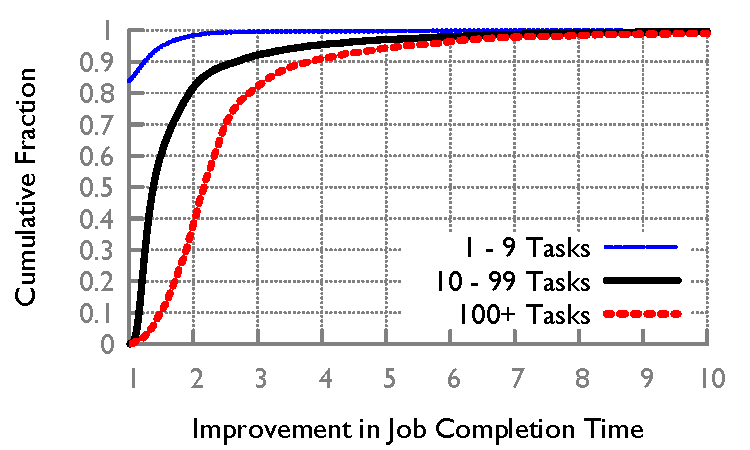
\includegraphics[width=0.45\textwidth]{figures/binpacked1-sep}
\vspace{-1.5in}
\label{fig:binpacked}
}
\hspace{0.2in}
\subfigure[] {
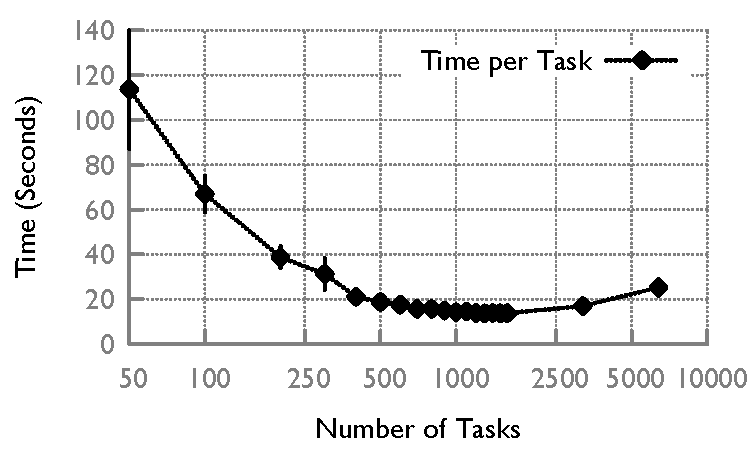
\includegraphics[width=0.45\textwidth]{figures/spark-skew-results}
\vspace{-1.5in}
\label{fig:sparkskew}
}
\caption{\subref{fig:binpacked} Improvement from perfectly balancing the total machine time for the
job across tasks. \subref{fig:sparkskew} Improvement from using tiny tasks in a cluster where 20\% of machines
take 21x longer to run each task. Error bars depict standard deviation.}
\vspace{-0.1in}
\end{figure*}

In this paper we present arguments and results motivating a move towards tiny tasks,
and we present preliminary design for a system supporting tiny tasks. In particular,
we propose a system that supports $100$ microsecond task launches, and an architecture
that allows most general applications to be expressed in terms of a set of tiny tasks.

\eat{We begin by quantifying the benefits of tiny tasks, using a series of simulations,
and application built on Spark\cite{zaharia2010spark} demonstrating the potential benefits
of using Spark. In Section~\ref{something} we outline the architecture for our system supporting tiny tasks, and
try and determine an appropriate task length based on task launch overheads, and other factors.
Next in Section~\ref{somethingelse} we discuss how to convert arbitrary jobs to better take advantage of tiny tasks, following
hich we discuss related work in Section~\ref{something}. Finally we conclude in Section~\ref{conclusion}.}

\section{Trends \& Motivation}

Common problems seen in datacenters. Probably need a graph for each one of these
\begin{myitemize}
  \item  Some tasks are very short/small and others are very large (in terms of
    resource usage) and long (in terms of time) \todo{Graph}.  
    Scheduling these is difficult; 

  \item Stragglers are exacerbated by the above problem~\todo{Graph}: if a task
    ends up on a machine with a large task consuming tons-o-resources, it will
    straggle

  \item Hot spots: there are hot spots in network usage, and also on machines
    that host popular data
\end{myitemize}

Make a table of problems caused by power-law distributions and papers about
them (should make this more concrete/compelling)

Datacenters and workloads are changing
\begin{myitemize}
  \item Focus is on main memory workloads, with need for low latency. Use the
    MapReduce$\rightarrow$Dremel$\rightarrow$Spark Streaming data here.
  \item Networks have grown to be fast making disk locality irrelevant. This
    means getting data from a remote location is fast. Further networks don't
    have a fixed overhead of transfer. Disk-based stuff uses 64MB to amortize
    that cost. \todo{Numbers ?}
  \item SSDs are becoming cheaper - Fast random access with low access time.
    With growing memory sizes + SSD, it is feasible to fetch most of the data
    without hitting the disk (local or remote).
  \item Need for low latency and ability to exploit fast-data access leads to
    tiny tasks
\end{myitemize}

\section{Benefits of Small Tasks}
\subsection{Running real-time and batch jobs together}
\kay{how can we quantify this?}
\subsection{How do small tasks affect stragglers?}
Breaking jobs into many waves of tiny tasks can improve completion time by 5x or more.  We assume task runtimes are exponentially distributed: some tasks take much longer than others due to resource contention on the machine, resource contention over the network, data skew, etc.  If tasks are all run in a single wave, the runtime of the job will be much longer than the mean task runtime, because the job is limited by the \emph{last} task to complete.  To measure the impact of breaking tasks up into a large number of tiny tasks, we assume jobs have a constant number of ''slots'' available, where a slot may represent a machine, or a fair share of the cluster allocated to the user who initiated the job.  we assume that if we break a task with mean runtime $x$ into k tiny tasks, each tiny task will have mean runtime $x/k$.  Figure~\ref{fig:outliers} demonstrates the impact of breaking a job with a single wave of tasks into $k$ times as many tiny tasks, for different values of $k$ (shown along the x-axis).  Response times are normalized relative to the response time for the job when run in a single wave.  We measure this impact for varying number of slots available to the job.  As expected, jobs with 1 slot see no improvement, but as the number of slots increases, jobs see as much as a 5x (eyeballed) improvement in response time from breaking tasks into tiny sub-tasks. This improvement justifies using a large number of tasks even if the overhead of starting a task is high; as long as the overhead of starting a task is less than 4x the task's completion time (we expect $<10$\% overhead), using tiny tasks will improve over running tasks in a single wave.

\begin{figure}[t]
\centering
\hspace{2ex}
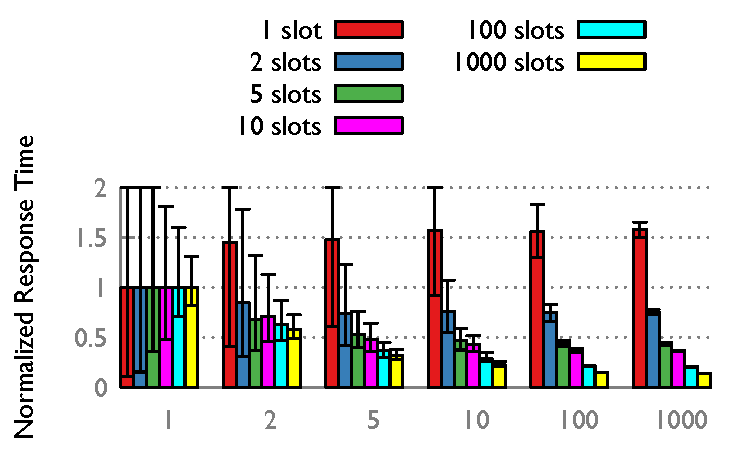
\includegraphics[width=0.5\textwidth]{figures/results_stragglers}
\vspace{-4ex}
\caption{Improvement in job completion time from breaking tasks into a large number of ``tiny tasks.'' \kay{need to fix 1-slot bars, which are screwed up, as well as nauseating colors}}
\vspace{-2ex}
\label{fig:outliers}
\end{figure}

TODO: use different original distributions of task duration

\subsection{How much do smaller tasks improve load balancing?}
two improvements on the load balancing front:
\begin{itemize}
\item File accesses: with smaller tasks, each task accesses a much smaller portion of a file.  In the context of Hadoop MapReduce, this would mean using much smaller HDFS file blocks.  With smaller blocks, the law of large numbers dictates that file accesses will be spread more evenly over machines than with large blocks.  To understand this affect, we use traces from Facebook's datacenter to obtain a distribution of the number of accesses per file.  We then randomly assign file blocks to machines, and measure the number of block accesses per machine, over 30 second intervals.\kay{should use smaller intervals? this would exacerbate affect, and you really care about how many accesses happen concurrently with yours, so 1s intervals could be realistic}  We divide files into smaller and smaller blocks (multiplier = 1 indicates block sizes equal to Facebook's current block size; multiplier = 10 indicates that we have block sizes 1/10th the size of Facebook's), to understand how smaller blocks improve load balancing.  With perfect load balancing, we would expect all machines to have the exact same number of file accesses.  Figure~\ref{fig:data_skew} demonstrates that even using 10 times as many tasks decreases 95th percentile machine load by 25\%\footnote{totally eyeballed from figure}.  \kay{we should simulate larger multipliers; my machine just died at 10}

\begin{figure}[t]
\centering
\hspace{2ex}
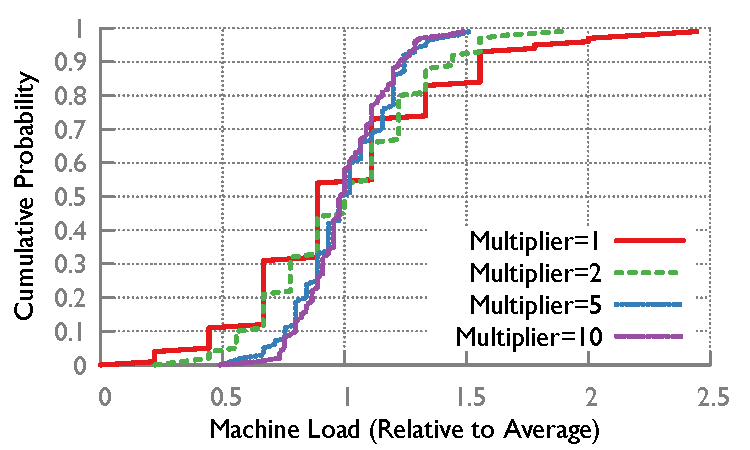
\includegraphics[width=0.5\textwidth]{figures/skew_results}
\vspace{-4ex}
\caption{Effect of decreasing file block size on the distribution of file accesses across machines.}
\vspace{-2ex}
\label{fig:data_skew}
\end{figure}

\item Network congestion: first, no huge flows (since all tasks are limited in how much data they use). This leads to essentially the same phenomenon as above.
\end{itemize}

\subsection{How do small tasks affect data skew?}
Many small tasks, so don't have to worry that one reducer (or other intermediate phase) has a ton of data.  Still need to worry about splitting very popular keys though...

\subsection{How does balance of tasks in a cluster (measured by queue length ?) change as we change granularity?}
\kay{Shivaram, what did you mean by this?}
\section{Architecting for Tiny Tasks}

\subsection{Design}

\begin{myitemize}
  \item API/Figure showing how tiny tasks look ? 
  \item Changes to the cluster scheduling arch. because of this.
  \item Example of how we take a Spark/Shark job and convert it to tiny tasks.
    Retro-fits into existing architecture seamlessly
  \item Some points about the data access we assume or build etc.
\end{myitemize}


\section{Challenges}

\subsection{How low can we go?}
Some back of envelope calculations here -- probably about 100ms. Maybe use
some of Josh's data for Spark.

\subsection{What about tasks that cannot be efficiently parallelized?}
\begin{itemize}
\item Simulated graph (based on FB traces) showing improvement as a function of
the percentage of tasks that can be parallelized
\item More extreme discussion of new framework that provides a distributed
scratch-space
\end{itemize}


\bibliographystyle{abbrv}
\bibliography{tiny-tasks}

\end{document}
